\section{Databasisontwerp}

\subsection{Inleiding}

Die databasisontwerp is 'n kritieke komponent van die stelsel, aangesien dit die
grondslag l\^e waarop die toepassing se data geberg en bestuur word. Dit lig
die res van die tegniese ontwerp van die stelsel in. 

Hierdie afdeling beskryf die struktuur van die databasis, insluitend die
tabelle, velde, en hul verhoudings. Die afdeling sluit ook 'n \ac{ERD} in wat
die visuele verhouding tussen die tabelle illustreer.

\subsection{Entity-Relationship Diagram (ERD)}

Die \ac{ERD} vir die stelsel is in \autoref{fig:erd_diagram} ingesluit. Dit
toon die tabelle, hul velde, en die verhoudings tussen hulle. Die diagram
bied 'n duidelike en georganiseerde voorstelling van die databasisstruktuur,
wat die ontwikkeling en onderhoud van die stelsel vergemaklik.

Die ERD volg die standaard benamingskonvensie waar tabelle in enkelvoudige
vorm gestoor word. Tabel name word in \textit{PascalCase} aangedui. In die Java
kode word die velde in \textit{camelCase} geskryf, maar in die
ERD en databasis word die velde in klein letters met \textit{snake\_case}
geskryf. Dit volg beide die Java konvensie in Java kode en \ac{SQL} konvensies vir
die databasis.

\begin{figure}[H]
    \centering
    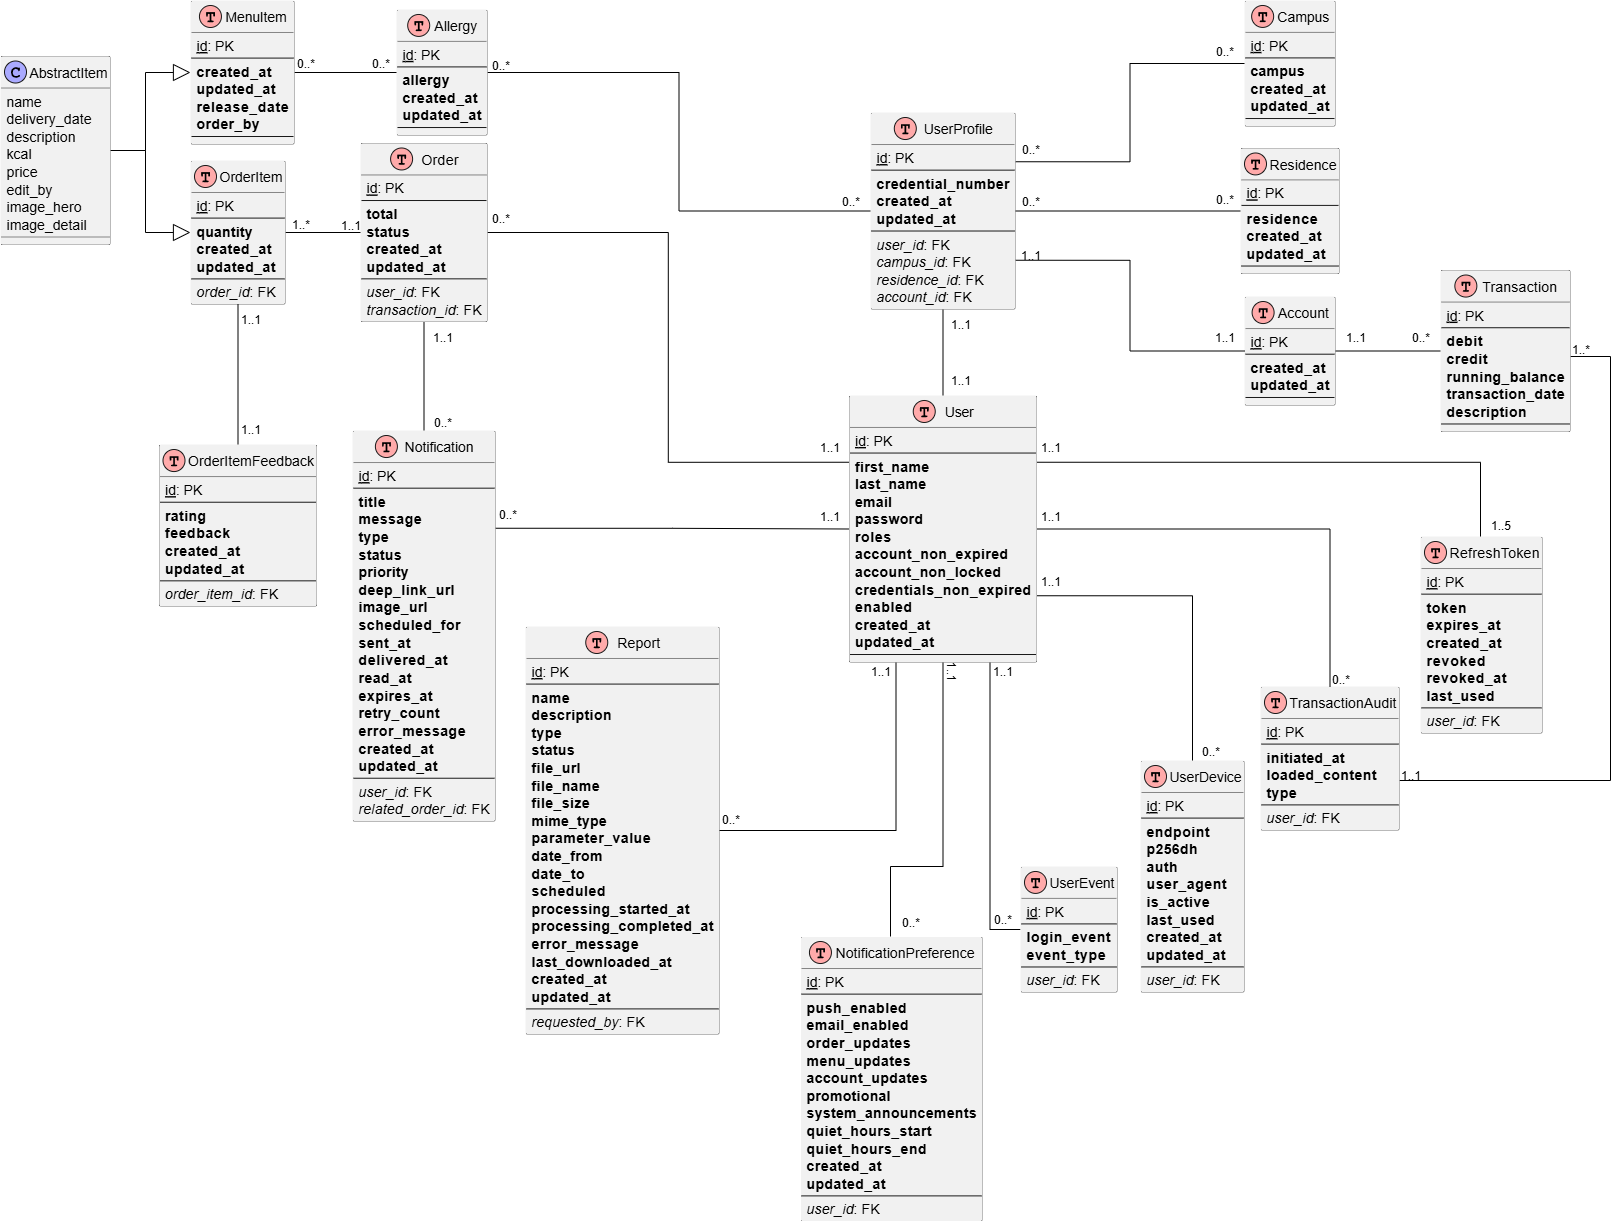
\includegraphics[height=\textwidth, angle=90]{figures/erd/erd.png}
    \caption{Entity-Relationship Diagram (ERD)}
    \label{fig:erd_diagram}
\end{figure}

Sentraal in die ERD is die tabel vir gebruikers, \textit{User}, wat die basiese
inligting van gebruiker rekeninge bevat, vir studente, personeel en
administrasie personeel. Dit sluit velde in soos naam, van, e-pos, die wagwoord
\textit{gehash} asook algene velde soos of die gebruiker 'n rekening gesluit
is, verval het, en dit sluit 'n \textbf{roles} veld in wat deur Spring se
\textit{Enumerated} annotasie gemerk word, waar Spring en Hibernate (Die databasisbestuur biblioteek) die beste
opsie kies vir die gekose databasis. Dit sal of 'n adisionele tabel skep
vir die gebruiker rolle of dit met \textit{one-hot-encoding} in die tabel self
berg.

Gebruikers kan ook 'n profiel hê, wat in die tabel vir profiele \textit{UserProfile}
geberg word. Hierdie tabel bevat velde soos studente- of personeelnommer
(credential\_number). Inligting soos kampus-ligging, koshuis indien van
toepassing, en allergene hanteer
deur 'n baie tot baie verhoudings te skep. Die \textit{link} tabelle word nie
getoon nie, omdat dit nie noodsaaklik is vir die begrip van die ERD nie.

Die stelsel bevat 'n tabel vir beskikbare items \textit{MenuItem}, waarvan bestel kan
word. Ons ondersteun ook 'n tabel vir bestellings, \textit{Order}, wat die
bestellings van gebruikers bevat, en 'n tabel \textit{OrderItem} vir die items
wat bestel is. Die leser sal oplet dat die tabel \textit{OrderItem} en
\textit{MenuItem} 'n super-tipe verhouding het met \textit{AbstractItem}. Die
ontwerp is so gekies sodata 'n item gekopi\"eer kan word as 'n bestelling
geplaas word, wat dataintegriteit verseker indien die oorspronklike item
gewysig word en historiese data behoue word.

Gebruiker profiele word met 'n een-tot-een verhouding met 'n rekening in die
rekening tabel \textit{Account} gekoppel. Die rekening tabel sluit nie 'n balans veld
in nie, omdat die balans vanaf die transaksies tabel \textit{Transaction} bereken word
deur om gebruik te maak van die \textit{running\_balance} veld. 

In lyn met industrie praktyk is rekords in die transaksie tabel is
onveranderbaar (immutable). Dit beteken om 'n transaksie te verwyder, moet 'n
nuwe transaksie geskep word wat die transaksie se teenoorgestelde waarde bevat.
Dit verseker dat die transaksie geskiedenis altyd beskikbaar is vir
ouditdoeleindes en dat die integriteit van die data behou word. Transaksies word
in 'n heelgetal vaste-punt formaat geberg, wat verseker dat dryfpunt foute vermy
word (\textit{floating point precision errors}) en dat die transaksies
akkuraat is.

Die stelsel beskik oor twee tabelle vir oudit doeleindes:
\textit{TransactionAudit} en \textit{UserEvent}. Die tabelle word gebruik om
transaksies en gebruikersaktiwiteite te monitor. Die transaksie oudit tabel word
gebruik om die oorspronklike bron van 'n transaksie te identifiseer, terwyl die 
gebruikersgebeurtenis tabel gebruik word om gebruikersaktiwiteite te monitor en
te analiseer. Hierdie tabelle help om die stelsel se sekuriteit en betroubaarheid
te verbeter deur 'n duidelike rekord van transaksies en gebruikersaktiwiteite
te bied.

Verder stoor die stelsel inligting rondom verslae in die \textit{Report} tabel,
asook kennisgewings in die \textit{Notification} tabel. Terugvoer word na die \textit{OrderItemFeedback} tabel gestuur, wat die terugvoer van gebruikers oor
bestelde items bevat. Hierdie tabel sluit 'n \textit{rating} veld in, wat die
gebruiker se beoordeling van die item bevat, sowel as 'n \textit{comment} veld
vir enige addisionele kommentaar. Hierdie terugvoer help om die kwaliteit van
die items te verbeter en bied waardevolle insigte vir die ontwikkelaars en
administrateurs van die stelsel.

Daar is taar tabelle vir tegniese doeleindes, soos die \textit{UserDevice},
wat inligting oor die toestelle van gebruikers sodat \textit{push-notifications}
gestuur kan word, en die \textit{RefreshToken} tabel, wat gebruik word om
gebruikers se sessies te bestuur. Hierdie tabelle help om die stelsel se
sekuriteit en gebruikerservaring te verbeter deur 'n veilige en betroubare
manier te bied om gebruikers se toestelle en sessies te bestuur.

